%!TEX root = ../main.tex
%=========================================================

\section{Overview}

There are 2 main operations, register(topic, self) and lookup(topic)
Every node acts as a advertiser and a registrar

\sergi{I would merge section 5 and 6 into a single section following the same structure of https://github.com/datahop/p2p-service-discovery/blob/master/doc/specs.md}

\subsection{Register}
Every registrar holds a \emph{topic table}, where it stores the incoming ads (\Cref{fig:registration}). Advertisers can send their requests to be added to the topic table on a registrar. Upon reception of a registration request, registrars compare it against ads already present in the table and calculates a request-specific \emph{waiting time}. The waiting time is determined by the diversity score of the incoming request and the occupancy of the topic table. The more the request differs from ads in the table, the lower waiting time it receives. It allows to maintain diverse content of the topic table, protects against hijacking the table by a small number of advertisers and ensures fairness towards less popular topics in the system. As the topic table gets filled, the returned waiting times increase as well. It spreads the load equally across registrars (loaded registrars issue longer waiting times and slow down the incoming traffic) and limits the total ad number in the table (bounding the registrar memory usage). 

A request is admitted to the table only if its \emph{accumulated waiting time} is higher than the returned waiting time. The \emph{accumulated waiting time} represents the total time the advertiser already waited for admission and is registered in \emph{ticket}. Tickets are immutable objects issued and signed by the registrars and includes the time of the initial request sent by the advertiser and the last waiting time returned by the registrar. Using the tickets avoids keeping additional state on registrars, while allows the advertisers to prove their \emph{accumulated waiting time}. 

If the \emph{accumulated waiting time} is lower than the waiting time, the advertiser receives a new ticket, waits for the remaining waiting time (waiting time - accumulated waiting time) and retries the registration. Importantly, the waiting time is re-evaluated every time the advertiser comes back. I.e., a previously returned waiting time is not an obligation for the registrar to admit the request at the specified time. The system guarantees that advertisers that waited long enough will eventually register at the topic table. 

\begin{figure}
    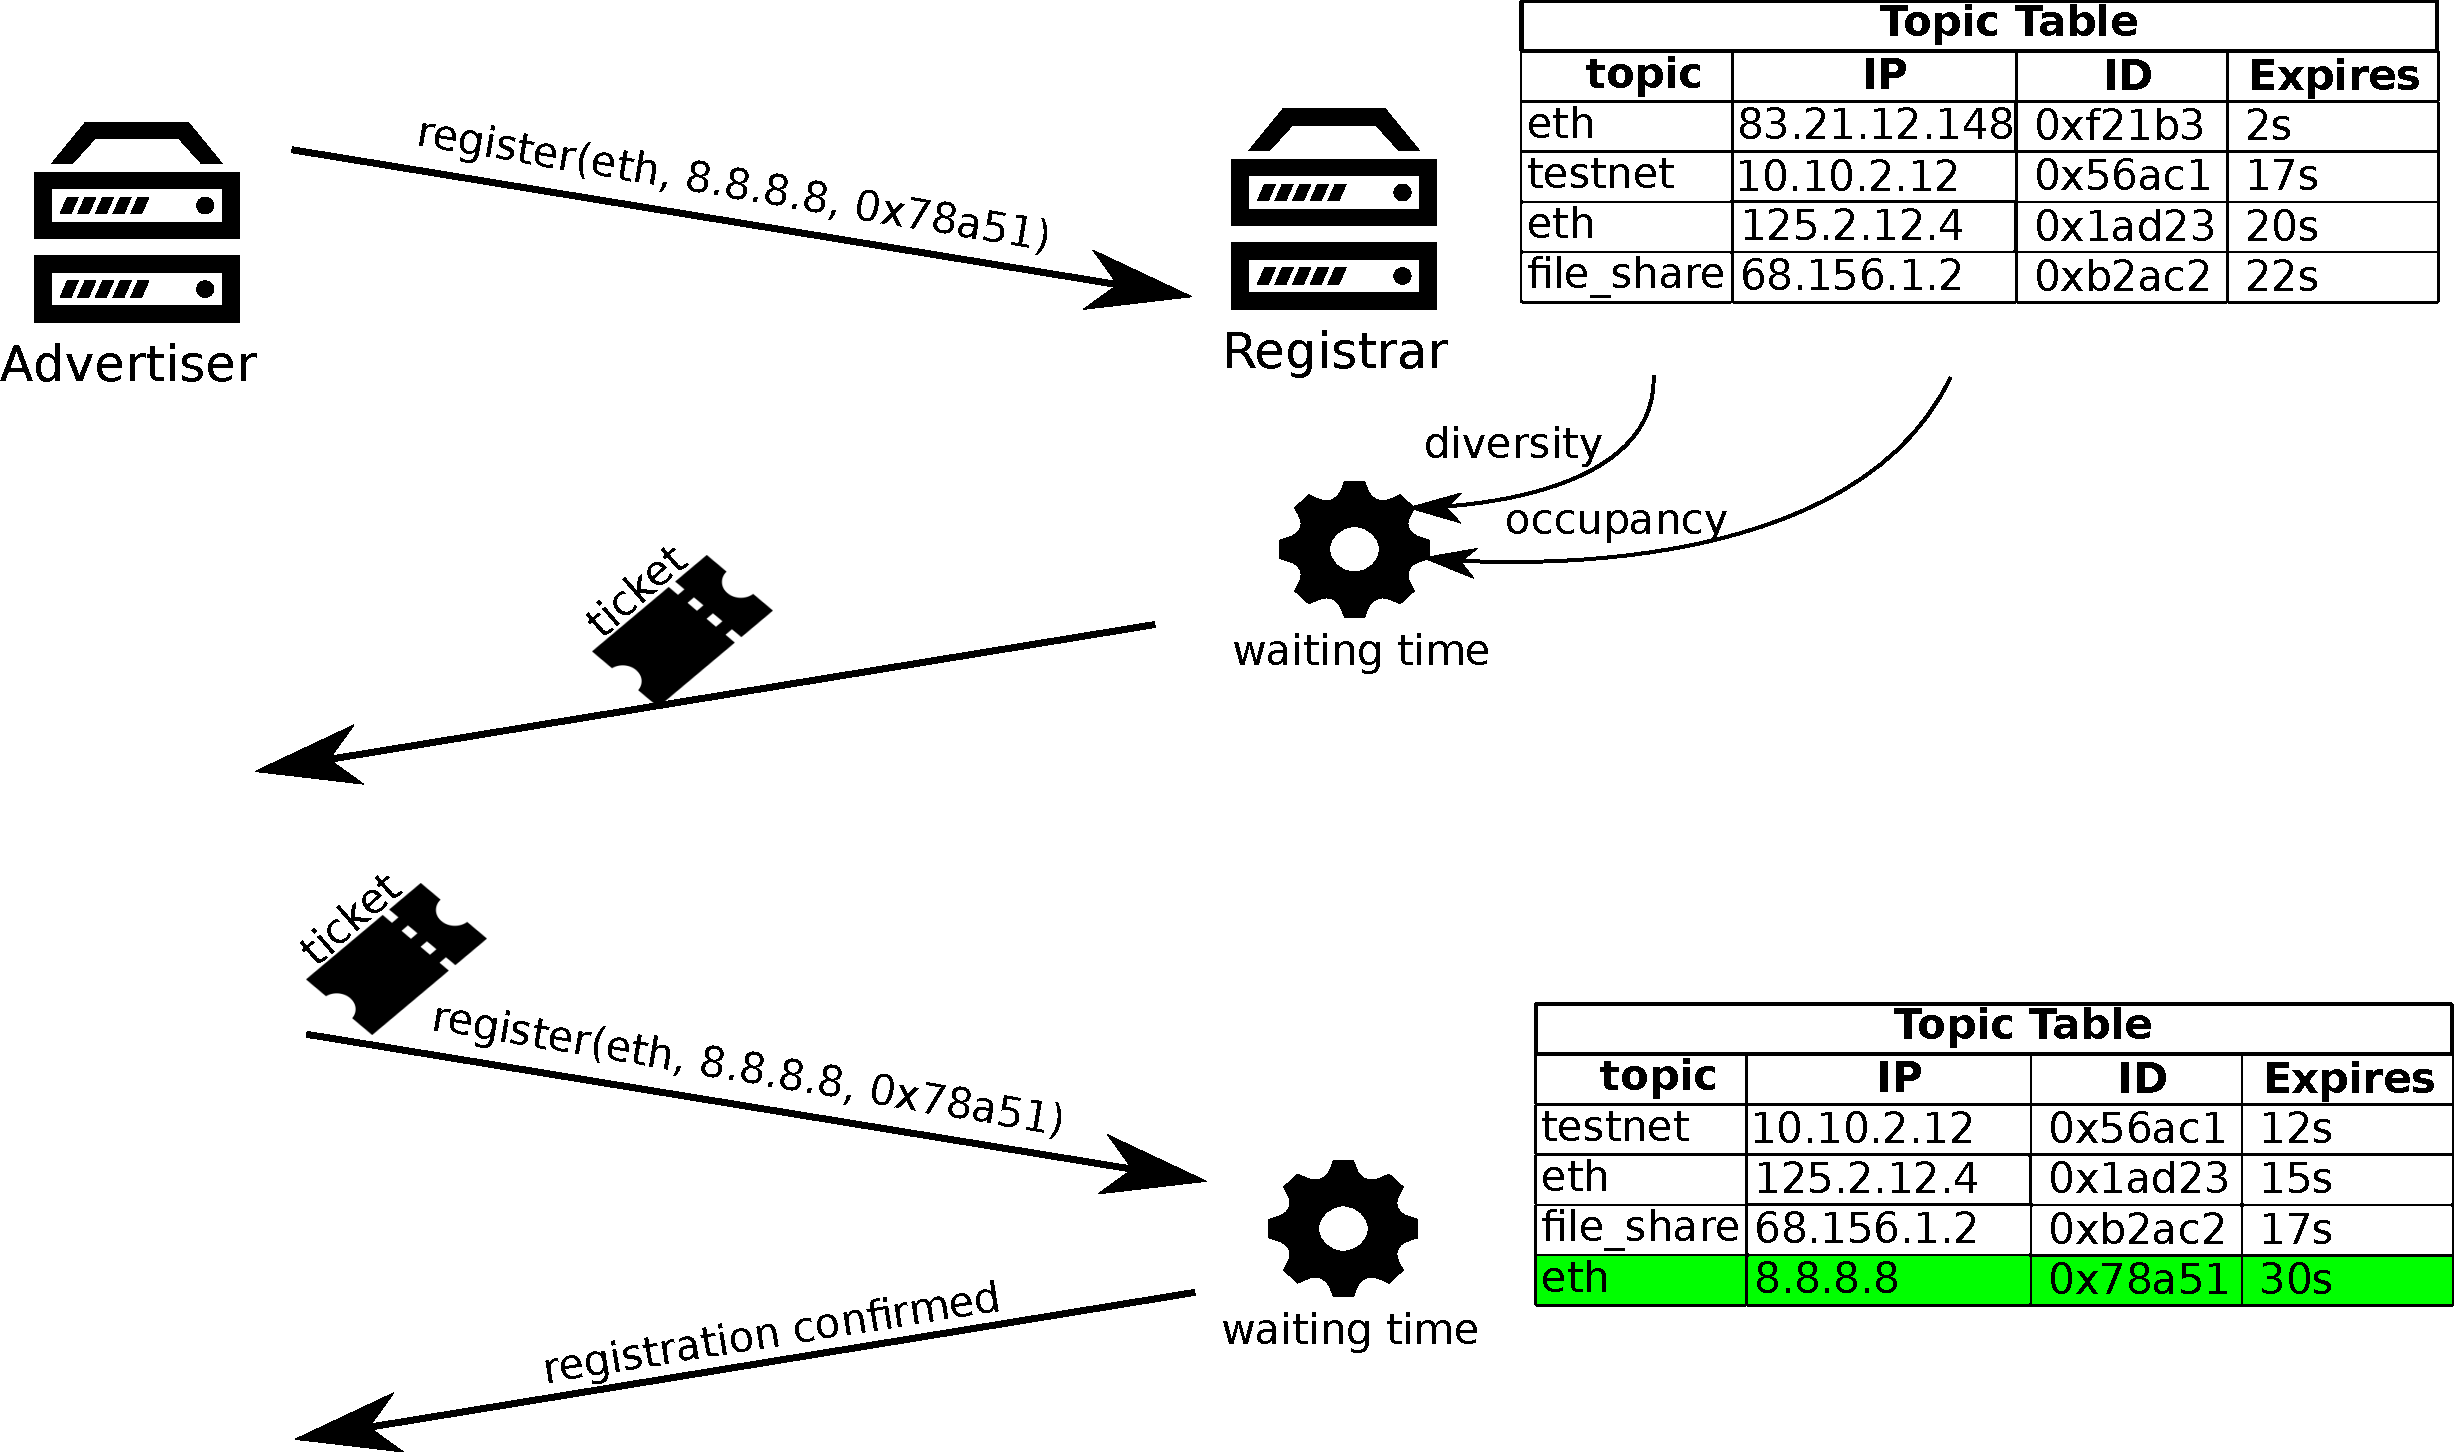
\includegraphics[width=0.5\textwidth]{img/registration}
    \caption{Registration process within one registrar.}
    \label{fig:registration}
\end{figure}




During the registration process, each advertiser tries to place its ads on multiple advertisers. It is required for availability as a single registrar can be malicious, attacked or simply leave the network. The advertisements should be placed in an unpredictable way to avoid targeted attack. On the other hand, the relevant registrar should be easy to find for searchers. Finally, we want to minimize the number of placed advertisement due efficiency reasons. 

At the beginning of each registration operation advertisers construct a \emph{ticket table} that will lead the process. The \emph{ticket table} is similar to the routing table. It is divided into buckets and holds peers in each bucket. However, buckets in the \emph{ticket table} indicate the distance from the topic hash the advertisers wants to register. The \emph{ticket table} is initialized with advertisers' peers from the DHT routing tables but organized in a different way (\Cref{fig:ticket_table}). The advertisers then tries to registers at a fixed number of registrars per bucket in the \emph{ticket table}. If a bucket holds more than the required number of registrars, a random subset is selected by the advertiser. The registration operation, places topic advertisements only on a small subsets of nodes (low overhead), includes randomness when choosing the registrars (attack resistance) and goes towards a specific point in the network indicated by the topic hash (efficient lookup).

Initially, advertisers might not know any nodes in buckets close to the topic hash\footnote{Especially if the topic hash is "far away" from the advertiser's ID}. When responding to registration requests, registrars also include a fixed amount of the closest peers to the topic hash the registrars know. The advertiser uses this information to progressively fill its ticket table. The closer the advertiser gets with the registration process, the more detailed information it receives. Similarly, to the basic DHT routing process, the registration operation eventually leads to the registrar that is the closest one to the topic hash in the entire network. 

\begin{figure}
    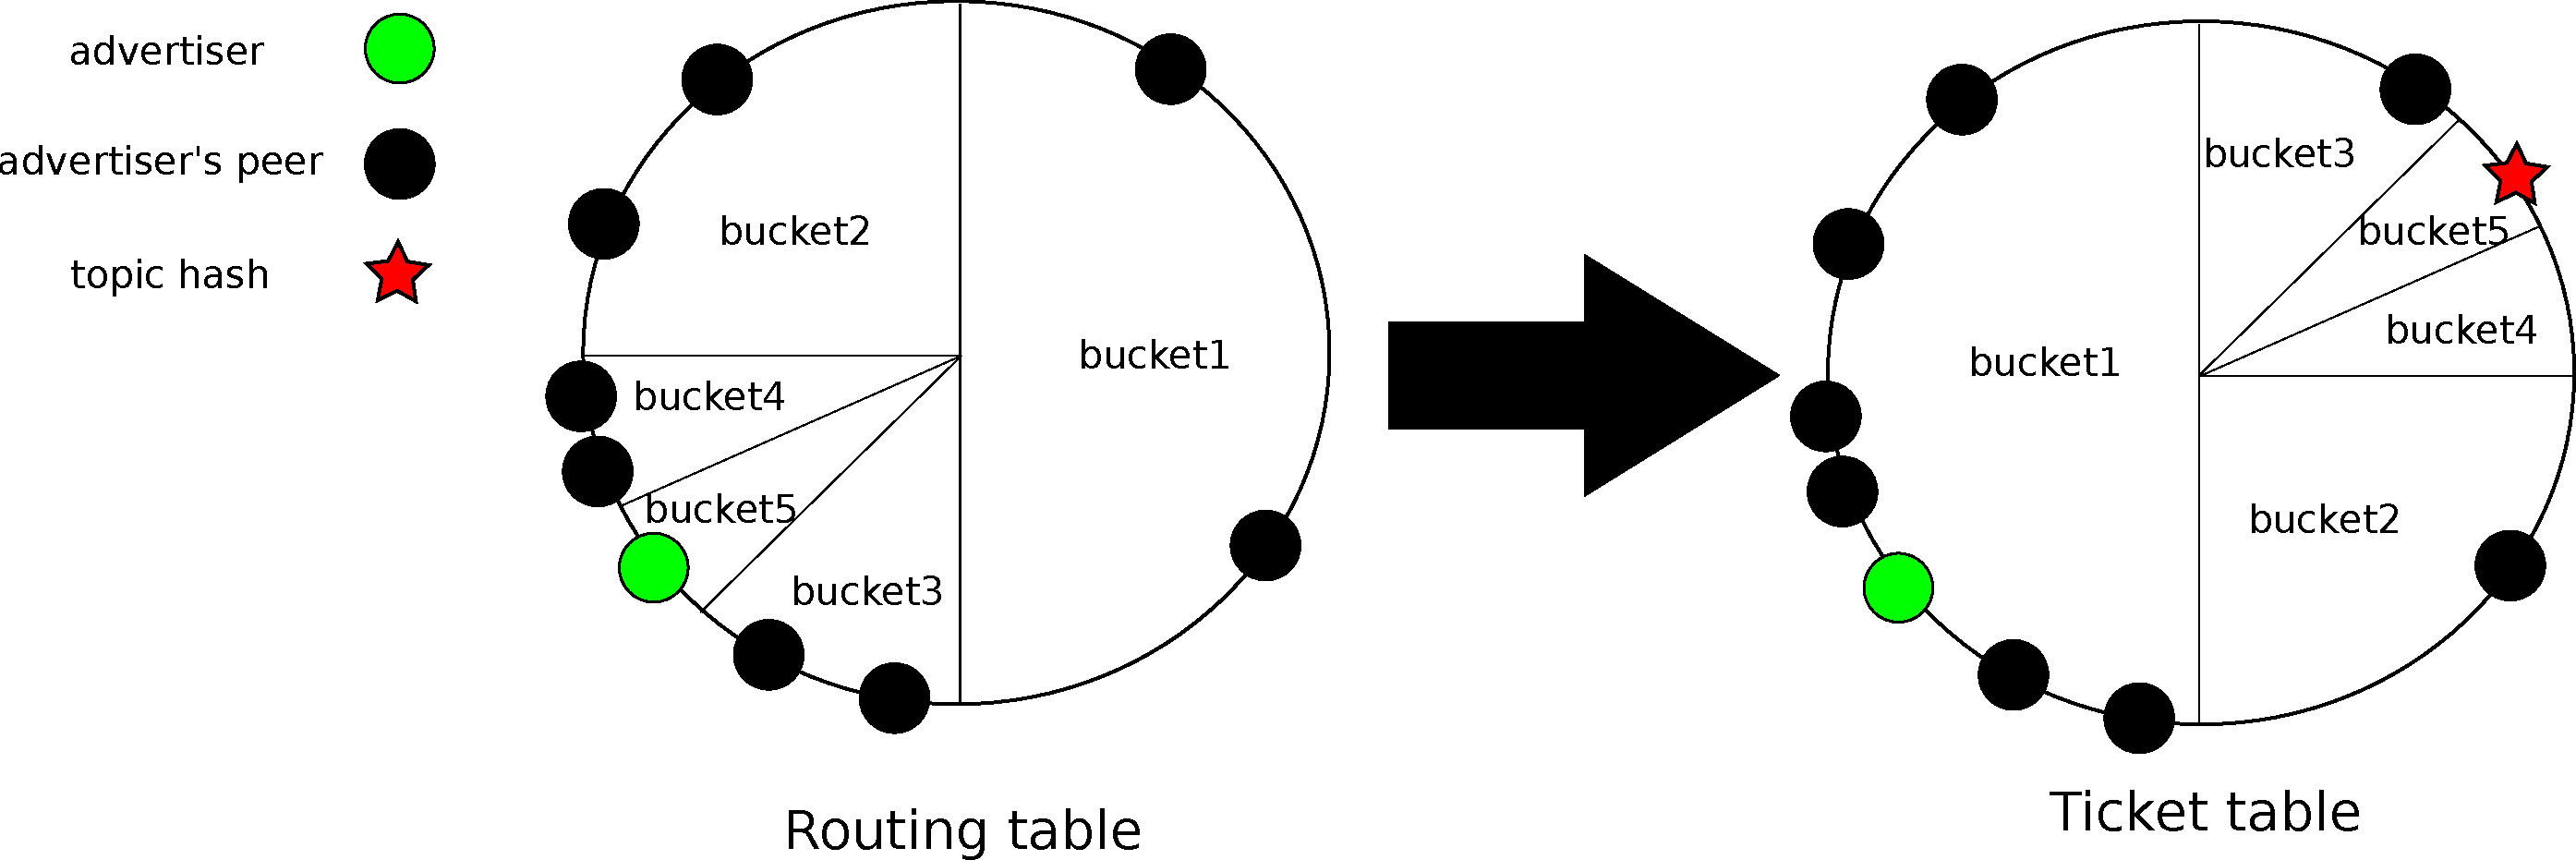
\includegraphics[width=0.5\textwidth]{img/ticket_table}
    \caption{Creation of ticket table from the routing table.}
    \label{fig:ticket_table}
\end{figure}

\subsection{Lookup}
The lookup operation closely mirrors the registration operation. The searcher starts by creating a \emph{search table}, organized in the same way as the \emph{ticket table} and determined by the topic hash. The searcher then starts the search from the furthest buckets in the search table and progressively moving towards buckets closer to the topic hash. A fixed number of random registrars is contacted for each bucket. Similarly to the registration operation, queried registrars respond with a list of the closest peers to the topic hash the registrars know of, allowing to progressively populate the search table. The search process stops when enough peers were found or when the closest registrar to the topic hash is reached. This approach allow searcher of popular topics to stop the process after a few queries without going all the way towards the topic hash and improves the load balance in the system. On the other hand, searchers of less popular topics are guaranteed to eventually discover all peer subscribed to their topic. 

